\documentclass[a4paper]{article}
\usepackage[T1]{fontenc}
\usepackage[utf8]{inputenc}
\usepackage{fancyhdr}
\usepackage{vmargin}
\usepackage{multirow}	
\usepackage{amsmath}
\usepackage{amssymb}
\usepackage{comment}
\usepackage{url}
\usepackage{graphics}
\usepackage{graphicx}
\usepackage{grffile}
\usepackage{color}
\usepackage{framed}
\usepackage{hyperref}
\usepackage{epsfig}
\usepackage{tikz}
\usepackage{float}
\usepackage{subcaption}
\usepackage{forest,calc}
\usepackage{tikz-qtree}
\usepackage{color}
\usepackage{colortbl}
\usepackage{capt-of}
\usepackage{booktabs}


\setlength{\parindent}{0pt}
\setlength{\parskip}{5pt}
\setlength{\headheight}{24pt}
\setlength{\headsep}{1.5cm}
\setlength{\footskip}{0cm}

\frenchspacing
\pagestyle{fancy}
\sloppy

\markright{headline}

% Kopfzeile
\lhead{\begin{tabular}{l}
		\textbf{Software Project}  \\
		\subtitle \\
\end{tabular}}

\rhead{\begin{tabular}{r} 
		\StudNameTwo\\
		\StudNameThree\\
		\StudNameOne\\
		\StudNameFour\\
\end{tabular}}


\newcommand{\subtitle}{\textbf{Singing Voice Synthesis with DiffSinger}}
\newcommand{\StudNameTwo}{\textbf{Jona Hoppe} - 7034173}
\newcommand{\StudNameThree}{\textbf{Hanna Helbig} - 7008726}
\newcommand{\StudNameOne}{\textbf{David Matkovic} - 7038335 }
\newcommand{\StudNameFour}{\textbf{Maximilian Schmidt} - 2560076}

\usepackage{setspace}  % Include the setspace package

\onehalfspacing
\begin{document}
\begin{titlepage}
    \centering
    \vspace*{1cm}

    {\LARGE\bfseries Saarland University \par}
    \vspace{0.5cm}
    {\Large Faculty of Language Science and Technology \par}
    \vfill

    % Title
    {\Huge\bfseries Singing Voice Synthesis with DiffSinger\par}
    \vspace{0.25cm}
    {\large\textit{A comprehensive Guide for Training a DiffSinger Model}\par}
    \vspace{1cm}

    % Subtitle or course context
    {\Large Winter Semester 2024/25 \par}
    \vspace{0.5cm}
    {\large Prof. Dr. Dietrich Klakow \par}
    \vfill

    % Student names
    {\Large\textbf{Project Members:}\par}
    \vspace{0.3cm}
    {\large\StudNameTwo\par}
    {\large\StudNameThree\par}
    {\large\StudNameOne\par}
    {\large\StudNameFour\par}

    \vfill
    {\large\today\par}
\end{titlepage}


	
	
	\tableofcontents
	\newpage
	
	%==============================================
	%================ Introduction =================
	%==============================================
	\section{Introduction}
 
 	Our work presents a method for emulating the vocal style of the late Chester Bennington, the former lead singer of Linkin Park. Our goal was to synthesize a new version of a song from the latest album “From Zero” using Chester Bennington’s distinctive voice. For this purpose, we used a pre-trained Singing Voice Synthesis (SVS) model called Diffsinger.
We compiled a dataset from the complete official discography of Linkin Park, including both studio and live recordings. This mixed dataset was deliberately chosen to expose the model to a range of different voice variations and production techniques over the years in order to make the model more robust.
After obtaining the data, we proceeded to isolate the vocal tracks with the help of several deep learning-based source separation tools. Subsequently, the extracted vocal tracks were segmented and aligned in preparation for the training. In the end, we used Reaper to mix the model’s output and combined it with the instrumental track of the album.

	\newpage
	
	%==============================================
	%================ Model Architecture =================
	%==============================================
	\section{Model Architecture}
	
	\subsection{Different approaches in VC}
	
	To generate recent tracks, but with the voice of Chester Bennington, we must introduce a method to convert or synthesize singing voices. Therefore, we briefly introduce the field of voice conversion, focussing on singing voice and singing voice synthesis. Voice conversion (VC) describes the transformation from a source speaker identity to a different speaker identity, while preserving the articulated linguistic content. During this process, different parameters of the voice, such as affect, emotion and accents are manipulated, to improve the naturalness and the similarity to the target voice. General breakthroughs that facilitated the study of voice conversion are the debut of computer based speech synthesis in the 1950s, the progress in digital signal processing during the 1970s and the recent advances in Machine Learning, especially induced by Neural Networks. \cite{Sisman2020} As a result, the difficulties of voice conversion have changed from solely generating natural sounding voices to more advanced applications, for example creating voices from scratch, that are not based on human training data. 
	
	Singing Voice Conversion (SVC) is considered a special case of VC, dealing with the conversion of sung voices. Additionally to the linguistic content, we want the pitch to be preserved as much as possible and focus more on the naturalness of the generated target voice (in terms of intonation, sound quality, timbre, energy and singing style). SVC faces similar challenges and difficulties as standard voice conversion but relies on further style parameters, which have to be trained. We contrast between parallel and nonparallel singing voice conversion: parallel SVC refers to models, that do a one-to-one conversion (which means they are only capable to convert the voice pair they trained on), while nonparallel SVC refers to any-to-one or any-to-any systems, where the target speakers are decoded via an additional input speaker-ID. There exist multiple well-known SVC models using different approaches, such as SOVITS which is combining Soft-VC and VITS, RVC which consists of an additional retrieval part and DDSP-SVC which uses a shallow diffusion mechanism. \cite{MediumSVC2023} A major problem SVC faces is data sparsity - due to copyright reasons we only have few published singing databases, often consisting of traditional folk songs.
	
	The less naive approach to generate a target voice is singing voice conversion (SVS). Singing voice synthesis models take the lyrics, the musical score and the respective duration as input and generate the audio file from scratch. During the training process the model predicts frame-level information of the target voice, which are then transferred to an audio signal by a vocoder. \cite{Cho2021} A prominent SVS system is the DiffSinger architecture.
	
	The singing voice conversion and the singing voice synthesis approach both come with advantages and difficulties, on which our model choice is based. SVC is a manipulation of the source audio and therefore often outperforms SVS models in preserving the singers expressiveness and naturalness, whereas SVS grant the user full control over the model and much more flexibility regarding the input songs (because it’s not reliant on existing performances). More flexibility increases the data and time consumption of synthesis models during training, which leads to higher computational costs compared with conversion models. 
	
	Another significant factor was the public data availability for our project. We have plenty of training data for our target voice (Chester Bennington), including 7 studio albums, 3 live albums and even more live performances - but we encounter a sparse data situation for Emily’s voice, where only a single album is published and even less audios are available, where both perform the same song.
	
	Regarding all advantages and factors mentioned above, we concluded that singing voice synthesis models fit our project better than the naive conversion approach. The sparse data situation for songs jointly performed by target and source singer, which is substantial for SVC training, forces us to focus on synthesizing methods. Furthermore we gain more flexibility and control over the model, which enables us to be more creative with the input data and gives light to a potential follow-up project - to generate new lyrics and songs with the voice of Chester Bennington.
	
	\subsection{Singing Voice Synthesis (SVS)}
	
	The breakthroughs in Deep Learning enabled novel possibilities for the generation of singing voices and in the past decade a variety of modern SVS architectures were proposed. While the majority of models are adapted voice conversion systems with additional singing-specific features, some of the proposed architectures introduce completely new concepts to Machine Learning and partly even influenced the field of voice conversion. Research focuses especially on models improving the naturalness of the output voice and models developed for low data situations. Subsequently, we travel through some of the most influential SVS models from the past decade to make our decisions transparent and comprehensible. \cite{Cho2021}
	
	Early systems are often based on hidden markov models (HMM), which consist of a rather plain architecture and comparatively simple to interpret. Consequently, the generated results are outdated nowadays and cannot reach the standard of recent models. \cite{Cho2021}
	
	The vast majority of recent SVS models use deep neural networks (DNNs) to preserve natural and expressive outputs. Important is the partition into submodules: an acoustic model, that is trained to predict acoustic and pitch related features and a neural vocoder that generates the audiowave based on the predicted information. This aspect of divide and conquer plays a decisive role in the success of neural models. Well-known DNN architectures are XiaoiceSing \cite{Cho2021}, which adopts the FastSpeech text to speech model and extends it with note duration and pitch information prediction; HifiSinger \cite{Cho2021}, a model generally based on XiaoiceSing, but using a GAN vocoder to prevent the model from over-smoothing; DiffSinger \cite{DiffSinger2021}, which improves the weaknesses of the previous models by introducing a diffusion probabilistic model (= gradually applies noise to the mel-spectrogram until the noise is gaussian distributed with subsequent denoising steps back to a mel-spectrogram).
	
	Apart from different approaches to enhance the target voice naturalness, low resource availability is a prevailing challenge in singing voice synthesis. Numerous models were designed to be more data efficient, requiring only small portions of training data, compared to the conventional models. The Sinsy \cite{Cho2021} model produces proper results with 1 hour of conditioned training data, partly due to a partition of the models architecture into further submodules. Zero shot models (for example StyleSinger and YourTTS) request merely minutes of training data to transfer voices in different languages or styles. \cite{Casanova2021},\cite{Zhang2024}
	
	Expressive and powerful models are also increasingly attracting the interest of large tech companies to market voice generators commercially. In 2022, Microsoft published its software DeepSinger \cite{Ren2020}, which conducts data mining on music websites to generate more training data. 
	
	\subsection{Model choice}
	
	Based on the presented architectures, we aimed to choose the model fitting our requirements the best. The model should produce natural audios and be capable of capturing the expressiveness of Chester Bennington’s voice. Further it should be comparatively easy to reimplement and well documented for research purposes. Data sparsity has solely been an issue for the source singer's voice, since Chester’s voice is published on numerous albums and publicly available. 
	
	Summarizing all models, we are of the opinion that the Diffsinger model meets our expectations the best and makes full use of the possibilities available to us, because it generates high-quality results and is widely documented with an active community of (non-commercial) users. Furthermore we are not reliant on computational and data limitations for our experiments and can therefore exploit the full potential of complex neural networks.
	
	\subsection{DiffSinger}
	The base model we used for our training and synthesizing is DiffSinger. It is an
	acoustic model, meaning it can map linguistik and symbolic input (like text or
	notes) into acoustic features, used to generate actual audio. Acoustic features
	include the most common feature mel-spectograms, but can also include linear
	spectograms, F0 and pitch contour, and energy. It is also a variance model,
	which is needed when trying to synthesize actual singing. A variance model
	models the acoustic variations, for example pitch, energy and duration of sound.
	The variance model predicts, based on the training data, how the voice features
	should vary over time, based on the input. To avoid long computation time and
	large resource needs, DiffSinger uses a shallow diffusion model. Traditional
	diffusion models generate data, by starting with pure, random noise, and step by
	step denoising it. This inference process is slow and takes many steps for just
	a single generated sample. The shallow diffusion model used by DiffSinger is a
	simpler and faster version of a full diffusion model. It uses fewer steps, but
	often starts with a better starting point (for example a prediction from another
	model). DiffSinger uses a non-diffusion model to predict a rough mel-spectogram
	for the synthesized data, and refines it using the shallow diffusion model. By
	using this technique, a lot of unnecessary steps, resources and computation time
	are saved. Not using another model to make a first prediction would cause the
	generated data to be a lot worse, since less steps are used and therefore less
	noise is removed.
	
	\newpage
	
	%==============================================
	%================ Preprocessing ================
	%==============================================
	\section{Preprocessing}
	
	\subsection{Initial Preprocessing}
	The initial phase of our project focused on preprocessing the audio data, which is a crucial step that encompasses several subtasks. The preprocessing aims at preparing the raw material for further analysis.
	
	\subsubsection{Data Acquisition}
	The first step before we could start with the preprocessing involved acquiring the songs that we wanted to use for our project. We wanted to ensure a diverse and representative dataset; thus, we searched for publicly available audio collections of Linkin Park. As we did not find a complete collection, we sourced the audios from YouTube. In total, we curated a corpus consisting of eight albums, each containing an average of 12 tracks. This collection formed the foundation for our subsequent processing and analysis steps.
	
	After collecting the data, we started with the preprocessing. Preprocessing is of critical importance for singing voice synthesis, especially when working with raw audio data, which is typically noisy and includes irrelevant or disturbing elements, such as instrumentals, audience noise, and silences, all of which can have a negative impact on model performance \cite{Kulkarni2023}.
	
	As we wanted to train the model to recognize the specific patterns of Chester Bennington’s voice, including his pitch, timbre and vocal fry, a good preprocessing is important to ensure that all relevant information is captured by the model and all irrelevant information (noise, other voices, instrumentals) is excluded to provide the best learning. Including instrumentals and noisy data would potentially lead to the model learning these unwanted features, resulting in a bad overall model output. This being said, we tried to preprocess our data, such that we excluded instrumentals and noise and included clean singing voice data, which was later passed through the model.
	
	
	\subsubsection{Segmentation}
	After the vocal extraction, the next step was to segment the data. Segmenting the audios into smaller chunks is important as it can significantly enhance the model’s performance and the reliability of the forced alignment that followed this step \cite{Rybach2009}. The quality of the alignment heavily depends on the segmentation, as a wrong segmentation will lead to a wrong alignment. The effectiveness of our model is, therefore, closely tied to the goodness of the audio segmentation. 
	
	The best way to ensure a good segmentation would be to do it manually, however, as our dataset is quite big, this would have been out of the scope of this project, so we searched for automatic segmentation methods.
	
	We tried different methods for automatic segmentation. We first used pydub, which is a Python library and a known powerful tool for preprocessing audio and text data, widely utilized in speech and text recognition applications \cite{Kulkarni2023}. We also tried pydub.silence, which is a module in the Python pydub library that provides functions to detect and handle silent segments in audio files. After that, we used Whisper, which is a powerful automatic speech recognition system developed by OpenAI \cite{OpenAI2022}. Whisper is trained on 680,000 hours of diverse, multilingual, and multitask data from the web, which makes it a robust model that can handle accents, background noise, and technical or domain-specific language, making it a suitable choice for our project, as speech clarity and variability are some of our main challenges. Whisper supports transcriptions for multiple languages. During the description, Whisper detects voice activity and attenuates background noise or music. In order for Whisper to work, PyTorch and ffmpeg must also be installed (those are its dependencies) \cite{Andreyev2025}. Whisper is not intended for real-time transcription and is designed to process audio containing at least one complete sentence, ideally under 30 seconds in length.
	
	Whisper's main challenge lies in balancing accuracy and resource efficiency, as it can produce hallucinated transcriptions and larger models demand high computational power, which limits their usability on resource-constrained devices \cite{Andreyev2025}.
	
	We also used whisper-timestamped, which is an extension of whisper and provides more efficient and accurate word timestamps. Whisper-timestamped uses a Dynamic Time Warping approach, which allows it to create word timestamps and a more accurate estimation on speech segments. As a result, the estimated start and end times of speech segments are more precise. Another advantage over the base model is that Whisper Timestamped can process longer files \cite{Andreyev2025}.
	
	Whisper-timestamped turned out to be the best model to segment our audios. It works with different model sizes: base, small, medium, and large. We used the small model as it was sufficiently well.
	
	Following an initial phase of trial and error, we implemented a custom script utilizing whisper-timestamped to segment our audio data. The script first verifies the file format, ensuring that only audio files (with the ending wav or mp3) are processed and that only those files whose names conformed to our naming convention (i.e., filenames containing either six or nine digits) were included. Once the appropriate files were selected, we used whisper-timestamped to generate segment-level transcriptions along with time-aligned boundaries. Most of the segments were fine, but some segments were extremely short (i.e., less than two seconds). To avoid these short segments and to enhance the usability of the resulting segments for annotation purposes, we introduced a minimum segment duration of four seconds. Thus, segments falling below this threshold were automatically concatenated with the subsequent segment to ensure that each snippet was sufficiently long to carry meaningful context for the automatic labeling. We also had some issues with hard cuts, where word endings were cut off too strictly. To mitigate this problem, we introduced a small buffer between consecutive segments (0.1s). This slight overlap helped preserve the natural flow of speech and ensured smoother transitions, which improved both the accuracy of our transcriptions and the overall quality of the audio snippets.
	
	
	\subsubsection{Manual Segmentation}
	
	To include more data and improve model performance, we additionally included two live albums in our dataset. As many segments contained screaming from the audience, we went through them and cut out unwanted parts manually with Praat, a tool for speech analysis and phonetic research.
	
	
	\begin{figure}[htbp]
		\centering
		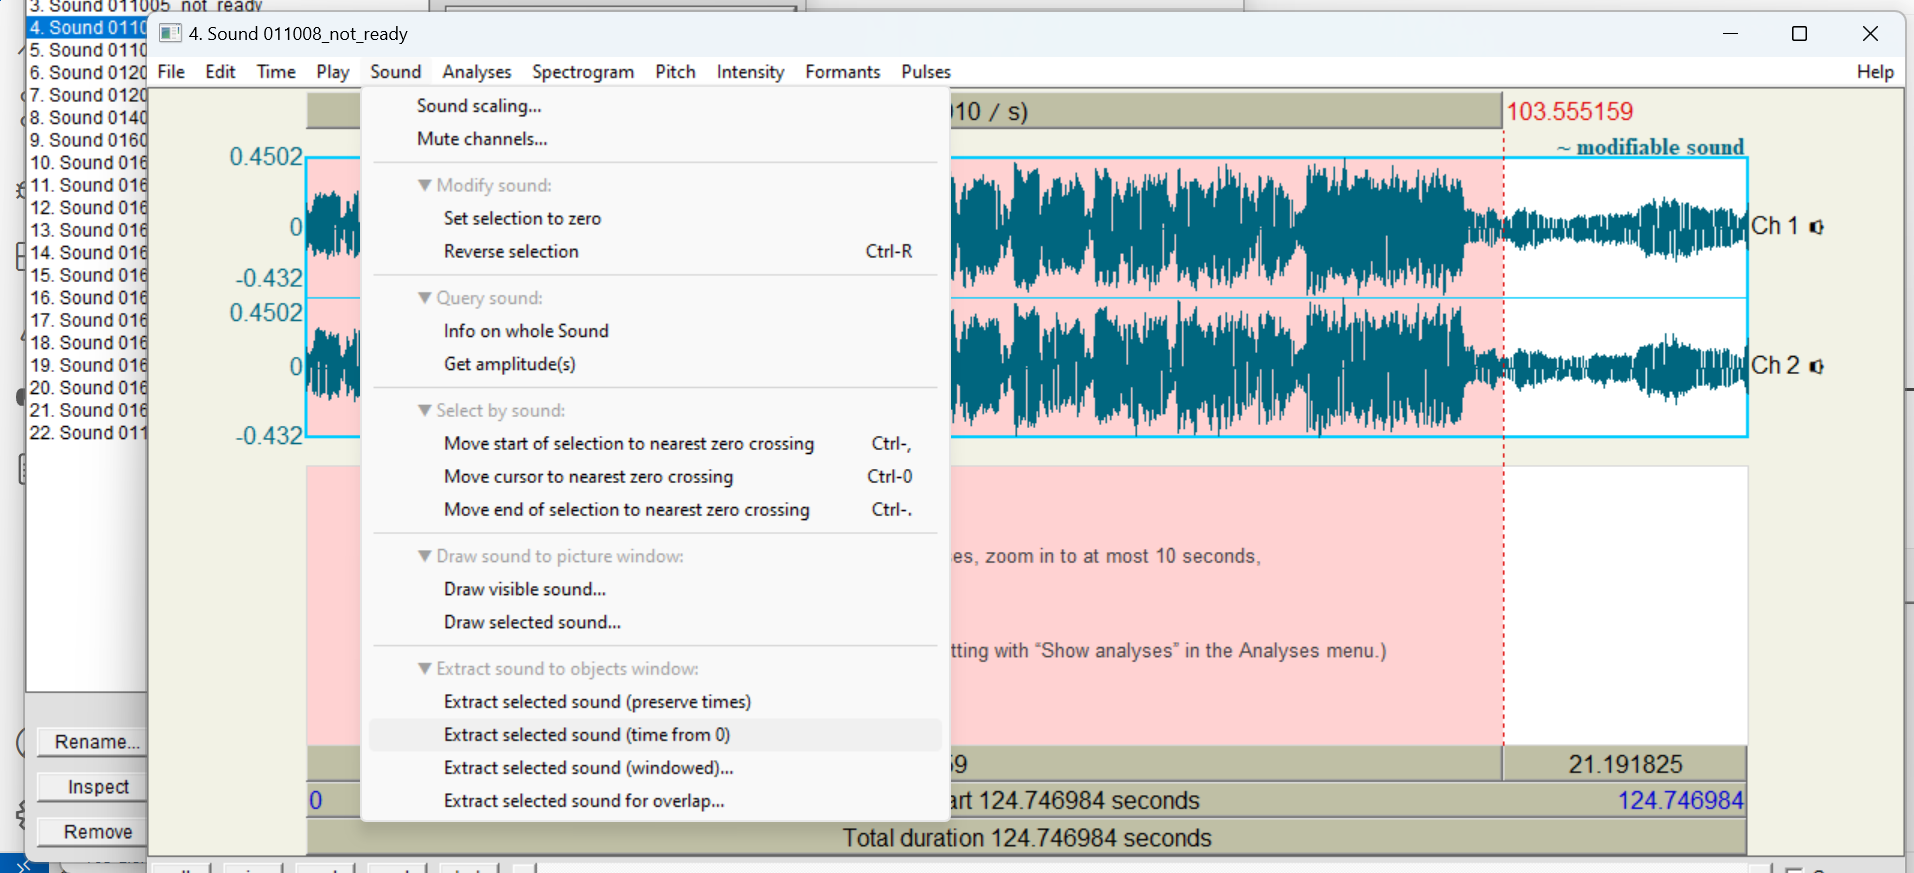
\includegraphics[width=0.5\textwidth]{graphics/cutting_noise.png}
		\caption{excluding noisy screams at the end of the audio snippet}
		\label{fig:bild1}
	\end{figure}
	
	After segmenting our data, we had to align our audio data with textual/phonetic annotations. Here, we encountered another challenge as some segments were silent, resulting in an error, thus, we excluded segments with zero variance before aligning the data.
	
	\subsubsection{Alignment Tools}
	We initially used the Montreal Forced Aligner (MFA), which is a widely recognized tool for automatic speech-text alignment. The MFA is built upon the Kaldi speech recognition toolkit. It is designed to provide robust phonetic segmentation by leveraging triphone acoustic models and speaker adaptation techniques \cite{McAuliffe2017}. MFA has been successfully applied to various languages and datasets; however, in our case, the MFA did not reveal convincing results. We attributed this to the fact that the MFA is primarily designed for spoken language, while singing poses some additional challenges, such as extended phonemes and pitch variations. 
	
	To improve alignment quality, we explored alternative tools and came across SOFA (Singing-Oriented Forced Aligner), which functions similarly to the Montreal Forced Aligner (MFA) but is specifically designed for singing voice. According to its Github page, SOFA offers simpler installation, better performance, and faster inference speed compared to MFA. After testing it on a few examples, we observed slightly improved results \cite{Greenleaf2001}; however, the alignments were still not consistently convincing. We continued our search and discovered LabelMakr, “a GUI tool to help users easily generate SVS phoneme-level labels” \cite{spicytigermeat} for singing voice synthesis (SVS), particularly intended for use with DiffSinger. While initial tests with a small sample also fell short of expectations, we observed that LabelMakr's performance significantly improved when it was applied to our full dataset, such that we ended up with some meaningful alignments that we used for our training.
	
	\subsubsection{Manual Alignment}
	In addition to our segmented audio snippets, we fully labeled two complete songs — Over Each Other and The Emptiness Machine — using LabelMakr, which we later used during inference. Since these full-song annotations were created after the short segments had already been labeled, the initial alignments were expectedly poor. To address this, we manually refined the boundaries: we shifted misaligned ones, added missing boundaries, and removed others — particularly SP (speech pause) and AP (aspiration pause) annotations, which frequently appeared in inappropriate positions.
	
	\begin{figure}[htbp]
		\centering
		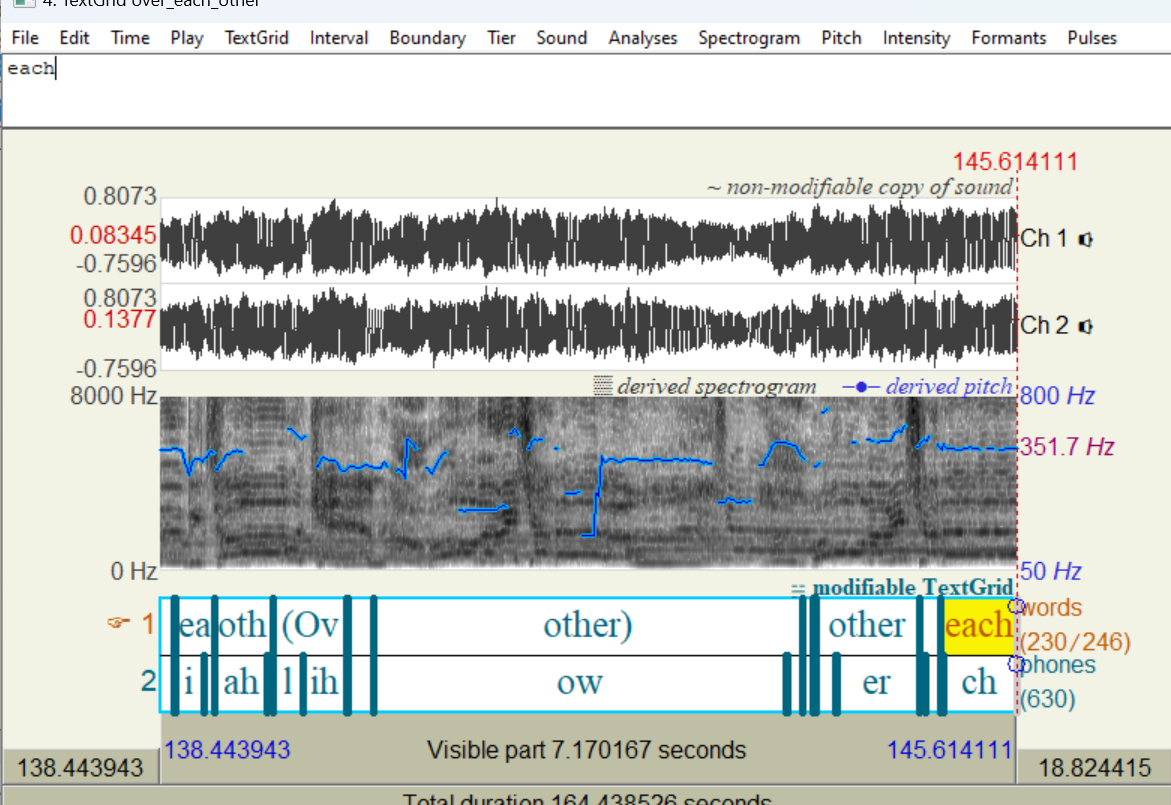
\includegraphics[width=0.5\textwidth]{graphics/bad_alignment.png}
		\caption{bad alignment}
		\label{fig:bild2}
	\end{figure}
	
	\begin{figure}[htbp]
		\centering
		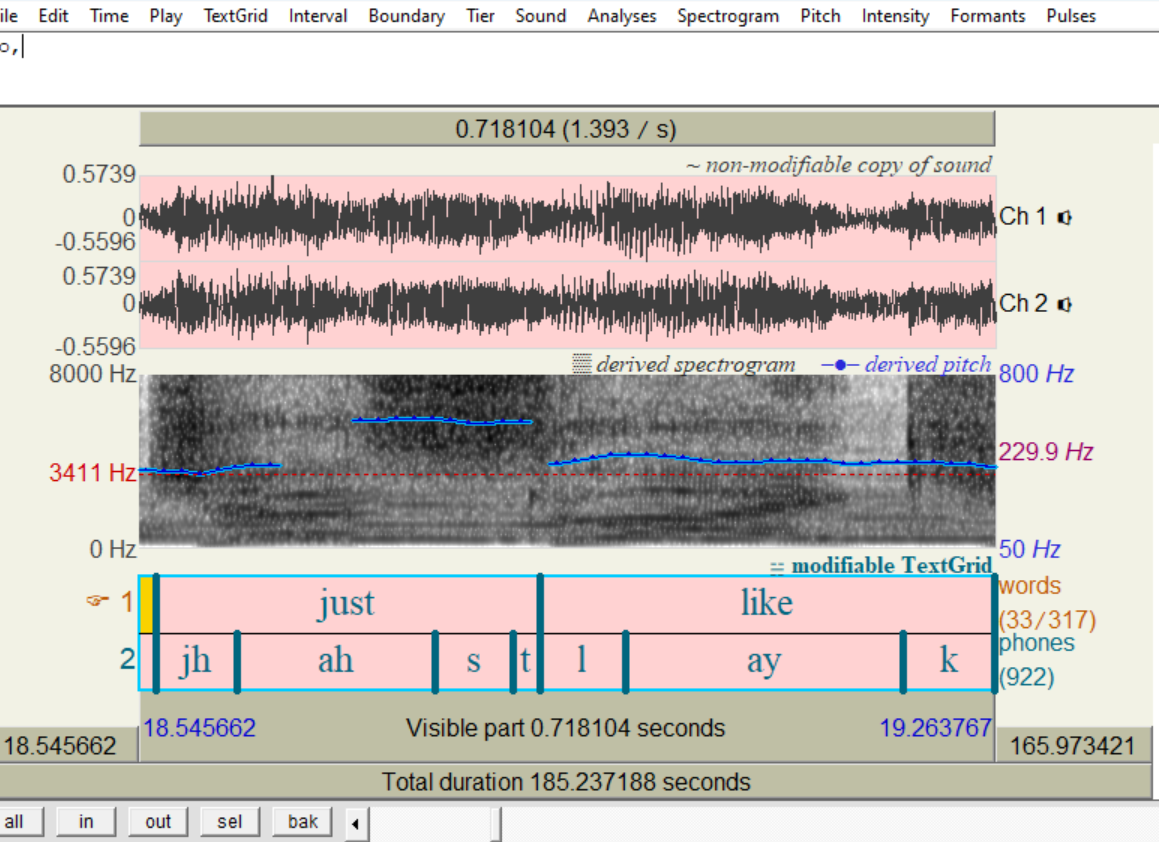
\includegraphics[width=0.5\textwidth]{graphics/manual_alignment.png}
		\caption{manual alignment}
		\label{fig:bild3}
	\end{figure}
	
	\subsubsection{Data Conversion with nnsvs-db-converter}
	We used the nnsvs-db-converter, a Python tool for converting vocal databases with HTS mono labels into DiffSinger format to make them compatible with variance models for predicting pitch and timing \cite{nnsvsdbconverter}. It handles sample segmentation by ensuring that each sample has a maximum length and an acceptable number of pauses between segments, and converts silent phonemes (e.g., sil, pau) to standardized representations (SP and AP for breaths). The script requires minimal external dependencies, making it easily accessible. In addition, it supports language definitions that specify vowels and liquids for better segmentation and timing handling, and it can estimate MIDI pitch and timing information for the use of variance models.
	
	In our project, we used this converter to convert our .lab files, which contained the phoneme alignments, into .ds files to ensure they were compatible with the DiffSinger framework and could utilize variance-based pitch and timing predictions.
	
	\subsubsection{SlurCutter Exploration}
	We also had a look into SlurCutter, which is a specialized tool that is designed to assist in the creation of datasets for DiffSinger. Its primary function is to edit MIDI sequences that are stored in .ds files to facilitate the preparation of data for variance model training \cite{openvpi}. However, it requires a lot of time and effort as this process is done manually, so we decided not to do it on a large scale.
	
	
	
	\subsection{Refined Preprocessing}
	As our initial training revealed noisy outputs, we decided to improve our dataset to enhance model performance. We began by manually manipulating two albums, where we removed segments that contained excessive noise, overlapping voices, or rap sections. The result was a cleaned subset of data, which we stored as our clear training data.
	
	To scale this cleaning process across the entire dataset, we wrote several scripts to automate the filtering process. First, we analyzed how different types of data snippets varied across the corpus. We manually selected representative examples of each category—screaming, multi-voice, clear voice, and rap—and stored them in separate folders to serve as our reference data.
	
	Initially, we attempted to map each song snippet to the category it was most similar to. However, this yielded inconsistent and often unreliable classifications, such that the categories had a large overlap and seemed to be meaningless. We then tried to identify dominant acoustic features that could meaningfully distinguish between categories. We found that fundamental frequency was a strong discriminator between screaming and clear singing. After analyzing our reference examples, we set a threshold of 230 Hz to filter out heavy screams and background noise—this removed many problematic segments while retaining the majority of clean vocals. The remaining screams in the clean voice examples were retained as they were less problematic than the really heavy ones and the background noises.
	
	To distinguish between rap and singing, we found that syllable rate is a suitable discriminator. Since our target singer, Chester Bennington, does not perform the rap sections, we applied a threshold of six syllables per second to exclude the fast-paced vocal segments.
	
	For segments with multiple overlapping voices, we explored various characteristics and thresholds, but none of them seemed to be a reliable discriminator. Therefore, we returned to the similarity-based approach—this time using only a single, well-chosen example per category to guide the classification, which surprisingly seemed to work better than with the bigger example set. While the categories were still imperfect, this method provided the most usable approximation.
	
	Ultimately, we combined the resulting clear voice set (without screams, rap, multiple voices) with other data to train three of our models (see model training).
	
	
	
	
	\newpage
	
	%==============================================
	%================ Training =====================
	%==============================================
	\section{Training}
	
	\subsection{Data Augmentation}
	
	Data augmentation describes the artificially increasing of the available training data to stabilize the training process, improve the performance and to diversify small and incomplete data sets. For this purpose, the existing training data is slightly modified and manipulated, reducing the  time and cost consumption that is often needed to generate real data. Previous studies showed that in voice conversion carefully designed augmentation is crucial. In particular additive noise and extensive data manipulation resulted in significant performance decreases and solely minor data changes achieved comparable accuracy. \cite{Slizovskaia2022}  For SVS, research groups proposed several different data augmentation methods with limited success. Experiment setups including cycle-consistent data augmentation or varying segment durations gained favorable results. \cite{Guo2022},\cite{Zhang2022} Also pitch shifting with a restricted range showed slight improvement of SVS models. \cite{Guo2022} Yet, none of the methods indicated a significant performance boost that outperformed all other methods. 
	
	Therefore, we augmented the data with two different approaches, first using the built-in application of the GitHub repository and second performing manual pitch and speed transformations.
	
	\subsubsection{Built-in Configuration}
	
	The openvpi DiffSinger repository allows two different ways of augmenting data, which can be controlled in the acoustic model’s configuration file. With the knowledge to augment data cautiously, we retained the preset parameters of the model. DiffSinger supports either fixed or random pitch shifting (default variant is fixed) ranging from [-5, 5] semitone divergence to the original data and time stretching in the range from half speed to double speed. \cite{openvpi-diffsinger}
	
	\subsubsection{Manual Augmentation}
	
	Data augmentation plays a crucial role in improving the fine-tuning and accuracy of speech attributes like pitch, loudness, and duration, enhancing the quality of AI-generated singing \cite{Morrison2024}.
	To enhance the diversity and robustness of our audio dataset, we implemented several data augmentation techniques: pitch shifting, loudness adjustment, noise reduction, and speed alteration. These methods are widely recognized for their effectiveness in improving speech recognition models by simulating speaker variations \cite{Morrison2024}. As singing is especially prone to these elements (e.g., pitch, loudness, and speed change drastically during a song), these augmentation techniques appeared to be especially useful for our purposes.
	
	\begin{itemize}
		\item \textbf{Pitch Shifting}: We wrote a script to adjust the pitch of each audio file by a semitone both upwards and downwards, creating two additional variations per original file. This technique helps the model become invariant to pitch differences as the pitch changes heavily between Chester’s different singing modes (e.g., compare harmonic singing versus screaming). We also tried to make more drastic pitch shifting, however, then the voice seemed to be too different from the original, so we did not include it in our model training.
		
		\item \textbf{Loudness Adjustment}: The audio files’ loudness was modified by increasing and decreasing the volume by 10\%. This approach aids the model in handling variations in speaking volume and recording conditions.
		
		\item \textbf{Noise Reduction}: We applied a noise reduction technique to suppress background noises such as ambient sounds and audience noise. This process aimed to enhance the clarity of the singing voice and thus, enhance model performance. However, we found that the denoising also suppressed the screaming parts quite a bit, so we decreased the initially high penalty to only 30\% noise reduction and used a less strict high-pass filter. For some parts, the screaming was still denoised too heavily, however, we used the denoised parts too to make the model more robust.
		
		\item \textbf{Speed Alteration}: The speed of the audio recordings was adjusted by $\pm$10\%, creating versions that are slightly faster and slower than the original. This method exposes the model to variations in singing rates, improving its ability to generalize across different singing tempos.
	\end{itemize}
	
	By incorporating these augmentation strategies, we aimed to increase the robustness of the model, leading to better overall performance.
	
	\subsection{Training Setup}
	
	The training setup and training organisation might seem less interesting and relevant at first, but the entire process (including the server usage) was particularly instructive for us and therefore deserves a section in the documentation. Opposing to Neil Armstrong - “That’s one small step for mankind, one giant leap for us” .
	
	The openvpi DiffSinger repository \cite{openvpi-diffsinger} offers significant advantages over the DiffSinger version that was implemented for the respective paper publication \cite{moon-diffsinger}; sufficient documentation is available, openvpi comes with an integrated variance module and the code readability strongly improved. The latter is particularly helpful, when we face problems that can only be solved by debugging.
	
	Initially we based our training setup on existing Google colab notebooks and other publicly available tutorials and used the procedures as orientation. Though  with colab notebooks, we encountered some fundamental and major problems relatively quickly, which forced us to build our setup from scratch. To avoid GPU usage limitations, we trained all our models on the LST servers of the Saarland University. \cite{lst-wiki}
	
	The LST cluster of the Saarland University uses HTCondor to schedule jobs and distributes them to free GPUs in incoming order. Users request the necessary computational cost for a job via submit files and transfer the file to be executed (must be a bash script). The dependencies are managed inside the bash script with an anaconda environment or in the submit file using a docker. For this purpose, we created an anaconda environment running on python version 3.8.20 and installed the necessary requirements following the DiffSinger installation guide. \cite{openvpi-diffsinger}
	
	Though HTCondor provides the possibility to distribute the executed job among several GPUs to decrease the running time, we restricted our training to 1 GPU (less potential to run into errors) and requested 16GB of GPU memory. After running for a maximum of 1 day, jobs get automatically kicked from the server by default. The image shows an example submit file that we used in our project.
	
	\begin{figure}[htbp]
		\centering
		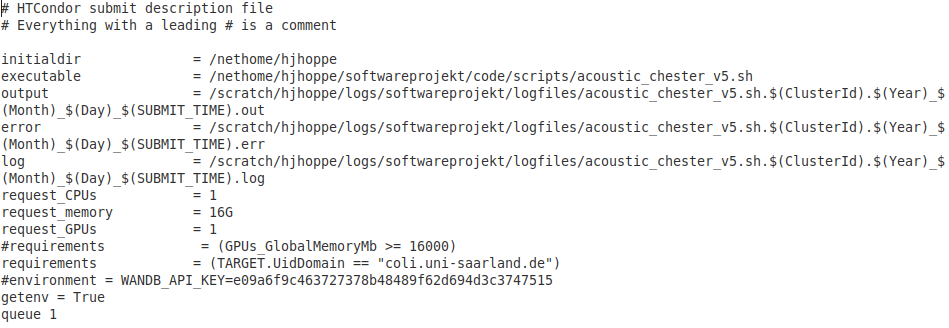
\includegraphics[width=0.5\textwidth]{graphics/submit_file.png}
		\caption{example submit file}
		\label{fig:submit_file}
	\end{figure}
	
	To gain control for optimal stopping points, we monitored the training process with tensorboard, which visualizes the current epoch, the course of training loss and validations loss and the results validation samples.
	
	\subsubsection{Problems}
	
	The configuration of the training setup caused us many problems for any number of reasons, which made the process an exhausting task. Often, installation and training guides from the internet were outdated and used DiffSinger versions that are no longer supported. Then for the first trial on our setup, we used Docker, which ultimately failed to search the python modules in the right folder, forcing us to find an alternative (anaconda environment). And once finished with the setup, trivias like a missing LST cluster specification delayed our project permanently. 
	
	\subsection{Training}
	
	We trained nine different versions of the DiffSinger model, applying various configuration alternations and providing datasets of different size and audio quality. All models were trained under equal conditions, which means that we always used the same conda environment for the runs and submitted, up to minor changes, identical bash scripts. The majority of training parameters remained constant and unchanged throughout the entire training procedure - therefore the configuration parameters in question are presented once at the beginning and apply to all training trials. Modified values (for example data augmentation) and integrated modules (for example the usage of a variance model) get specified in the section of the particular run. 
	
	The main architecture of the DiffSinger model is trained to predict mel-spectrograms out of the input data, but that is not exactly what we challenged ourselves. To generate audio files from the mel-spectrograms a vocoder is necessary. For a start we stuck to the HifiGAN vocoder recommended in the openvpi DiffSinger support, which we ultimately fine-tuned on Chester’s voice (training see below in the section vocoder). 
	
	The repository offers several built-in models operating as pitch extractor and harmonic-noise separator as well, recommending RMVPE for extracting pitch and Vocal Remover (VR) to separate the harmonic and aperiodic parts of the singer's voice. For the shallow diffusion configuration again we were oriented strongly towards the given guide, copying the preset parameter values. 
	
	Another relevant decision, to minimize the training loss and presumably improve the mel-spectrograms, is the right choice of optimizer and learning rate. Previous experiments and the paper itself achieved promising results with the AdamW optimizer and different learning step sizes. So there was no reason for us to integrate different optimizers than AdamW and unless otherwise stated we set the learning rate to 0.0006. 
	
	To preserve high-quality audio outputs we used as sample rate 44.1 Hz, with a hop size of 512 (which is the step length of mel and feature extraction) and a balance between frequency resolution and efficiency during the mel-spectrogram extraction, setting 2048 for the Fast Fourier Transform size.
	
	\subsubsection{Vocoder}
	
	Another tool to enhance the overall performance, is fine tuning the vocoder on the target voice. This should in theory improve the transformation process from mel-spectrogram to audio, in particular preserving the singer identity characteristics and the singing style. For this purpose, we trained the recommended HifiGAN model checkpoint on the cleaned (hand segmented) dataset for a few epochs to personalize the vocoder. The AdamW optimizer updated the vocoder parameters with learning rate 0.0001 and batch size 6. Different to the DiffSinger model, the HifiGAN vocoder was fine-tuned using parselmouth as pitch extractor. During training we observed convergence of the validation loss relatively quick after around 2000 epochs. 
	
	\subsubsection{Model 1 (small)}
	
	\begin{figure}[htbp]
		\centering
		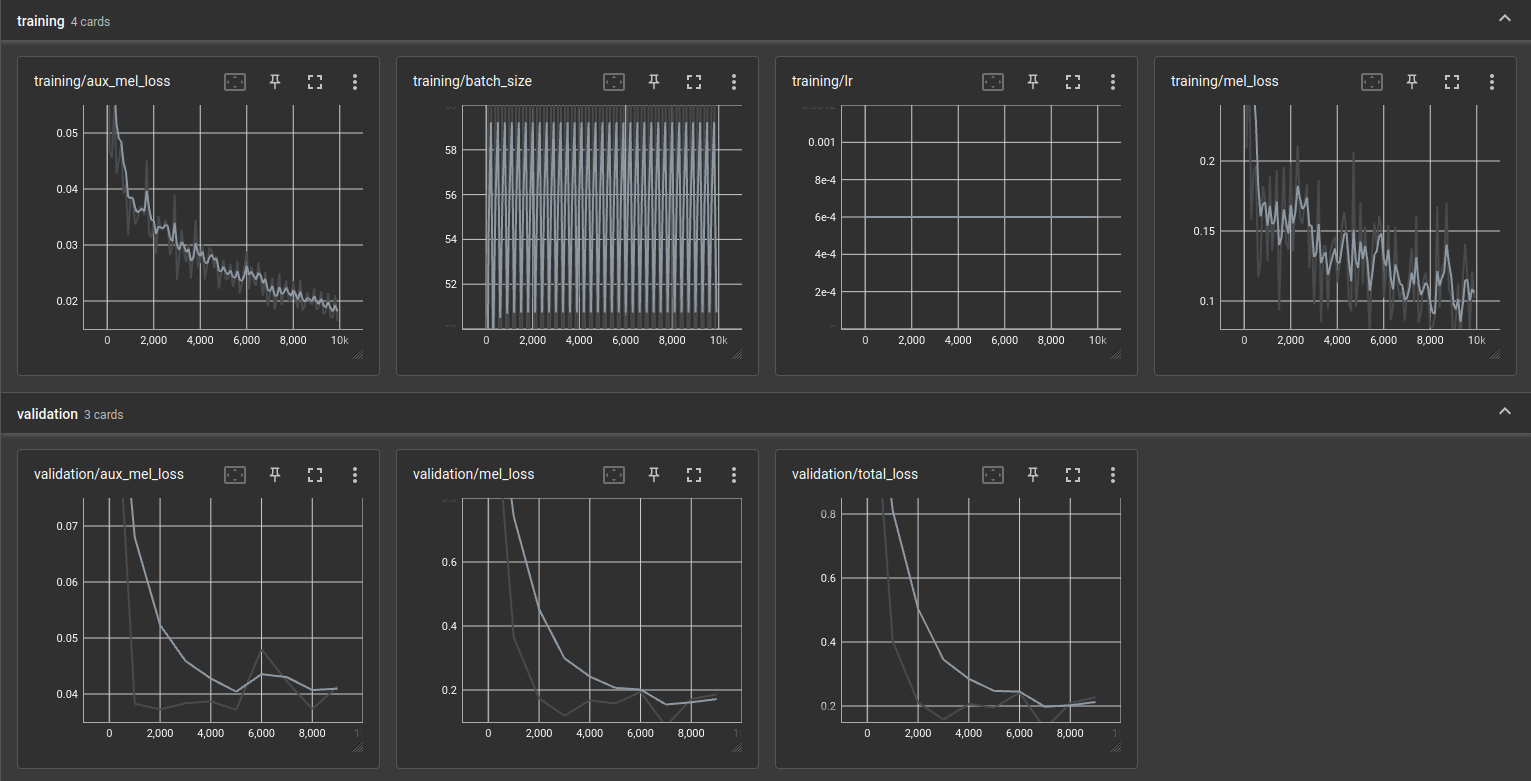
\includegraphics[width=0.5\textwidth]{graphics/v1_training+testing.png}
		\caption{training and validation loss of model 1}
		\label{fig:model1}
	\end{figure}
	
	The first generated model served primarily as a test trial to check whether the entire workflow, from extracting input data to generate outputs, functions. Unsurprisingly we kept the standard configuration from above, without using any form of data augmentation or fine tuning and without using a pretrained variance model. The dataset consisted of all available studio albums and we used 6 segments for validation and we used a batch size of 64. We stopped the training after roughly an hour and 9900 trained epochs, while the training loss was still on decline - though the validation loss already stabilized around 0.04 (as displayed in image \ref{fig:model1}). In the following we will refer to this model as small.
	
	\subsubsection{Model 2 (small)}
	
	\begin{figure}[htbp]
		\centering
		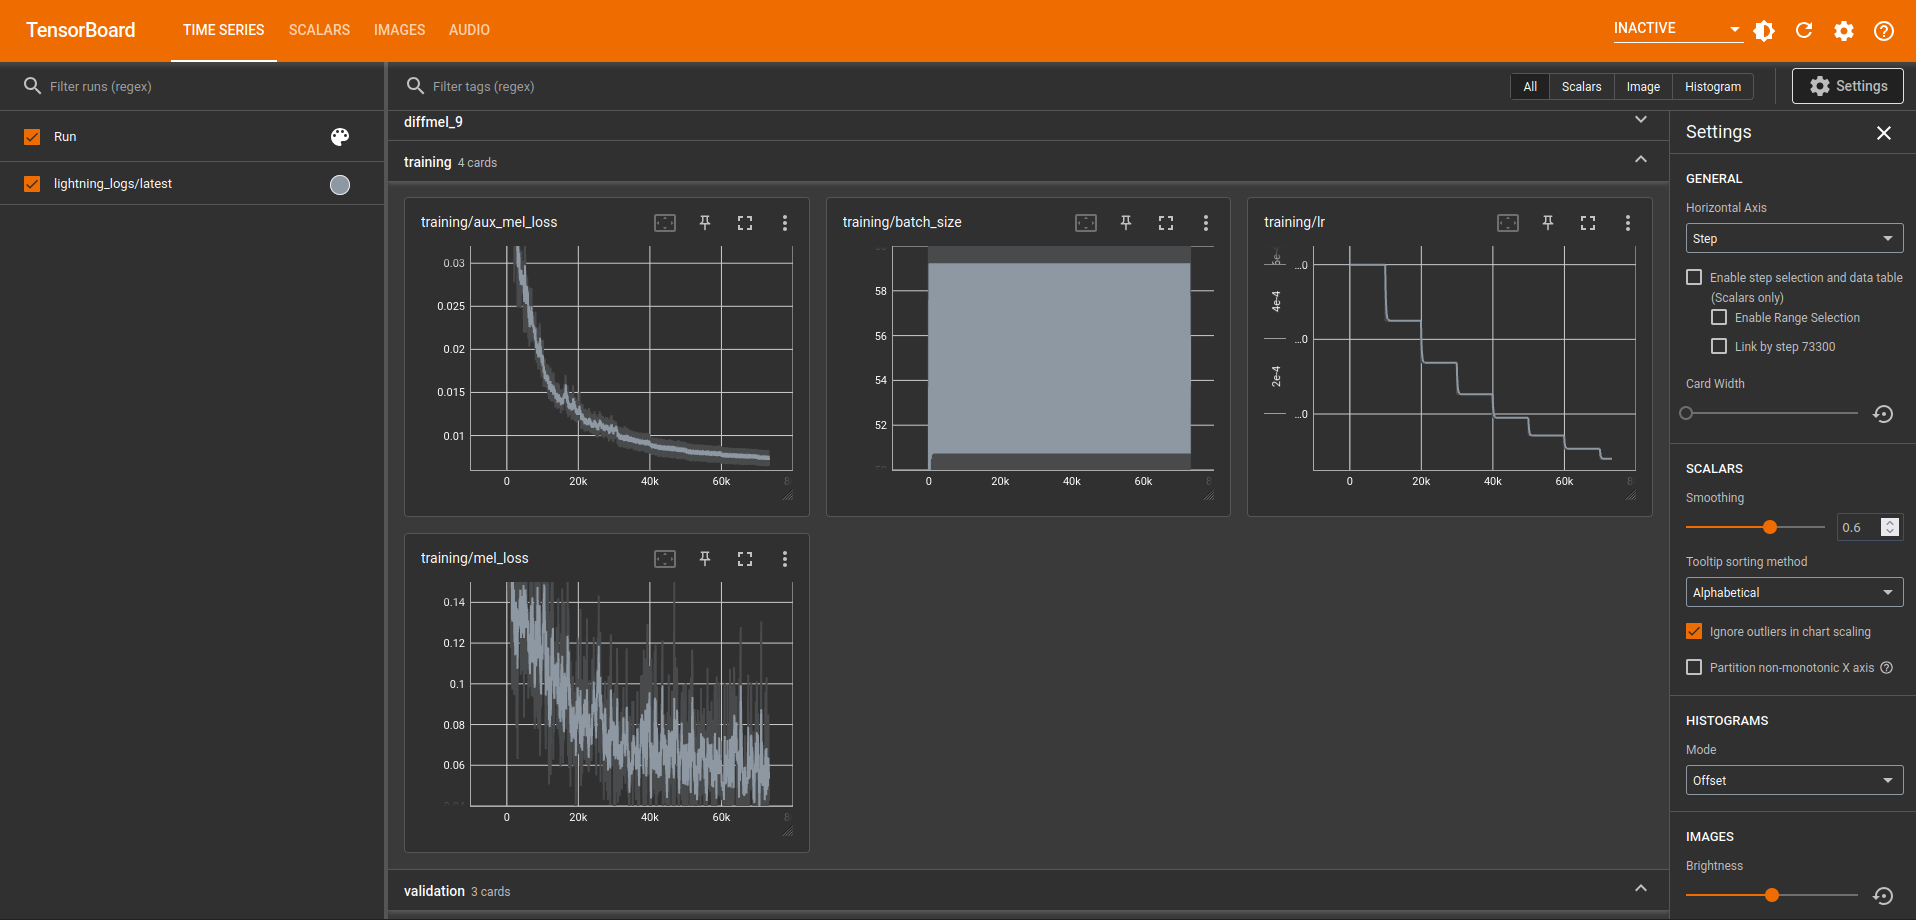
\includegraphics[width=0.5\textwidth]{graphics/v2_training.png}
		\caption{training loss of model 2}
		\label{fig:model2train}
	\end{figure}

	\begin{figure}[htbp]
		\centering
		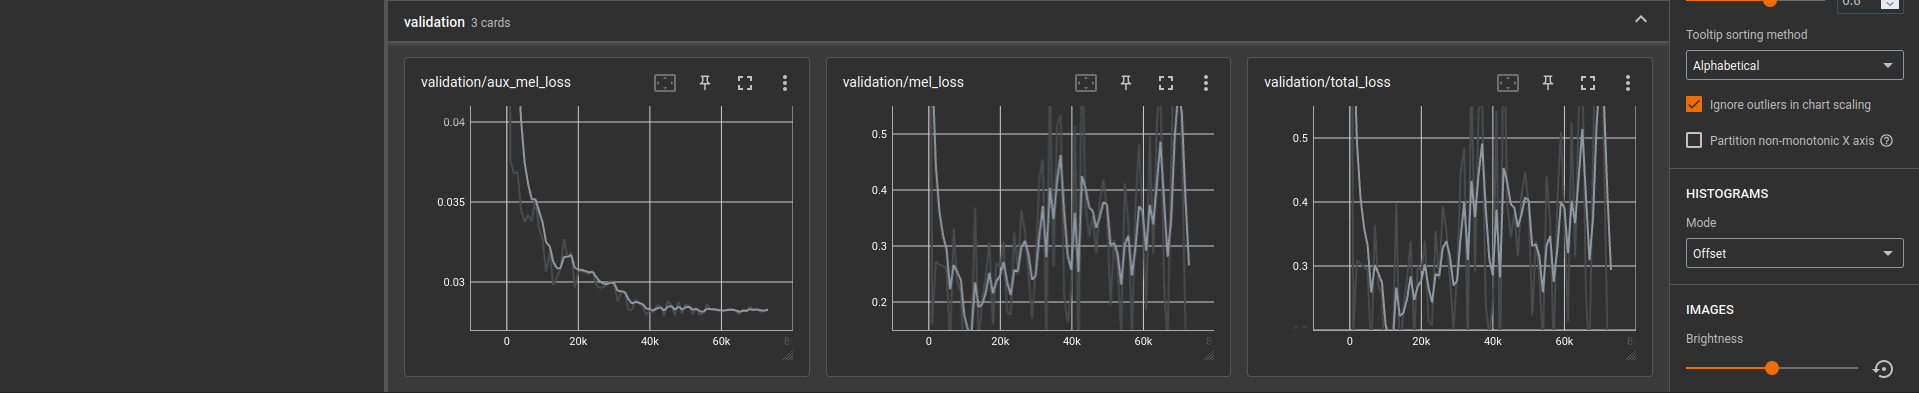
\includegraphics[width=0.5\textwidth]{graphics/v2_testing.png}
		\caption{validation loss of model 2}
		\label{fig:model2val}
	\end{figure}
	
	The second generated model serves as an extensive version of the small model in the section above. All configuration and hyperparameters were transmitted with the only difference of a longer training duration until the training loss stabilizes. After a little more than 70k epochs, the aux mel training loss decreased to 0.009 and the mel training loss reached the minimum of 0.06. Worth mentioning is the increasing fluctuation of the validation loss, starting after reaching the minimal value (see image \ref{fig:model2val}). Due to no subjective improvement of the model compared to Model 1, this version is not sustained in the following evaluation process. 

	
	\subsubsection{Model 3 (large)}
	
	\begin{figure}[htbp]
		\centering
		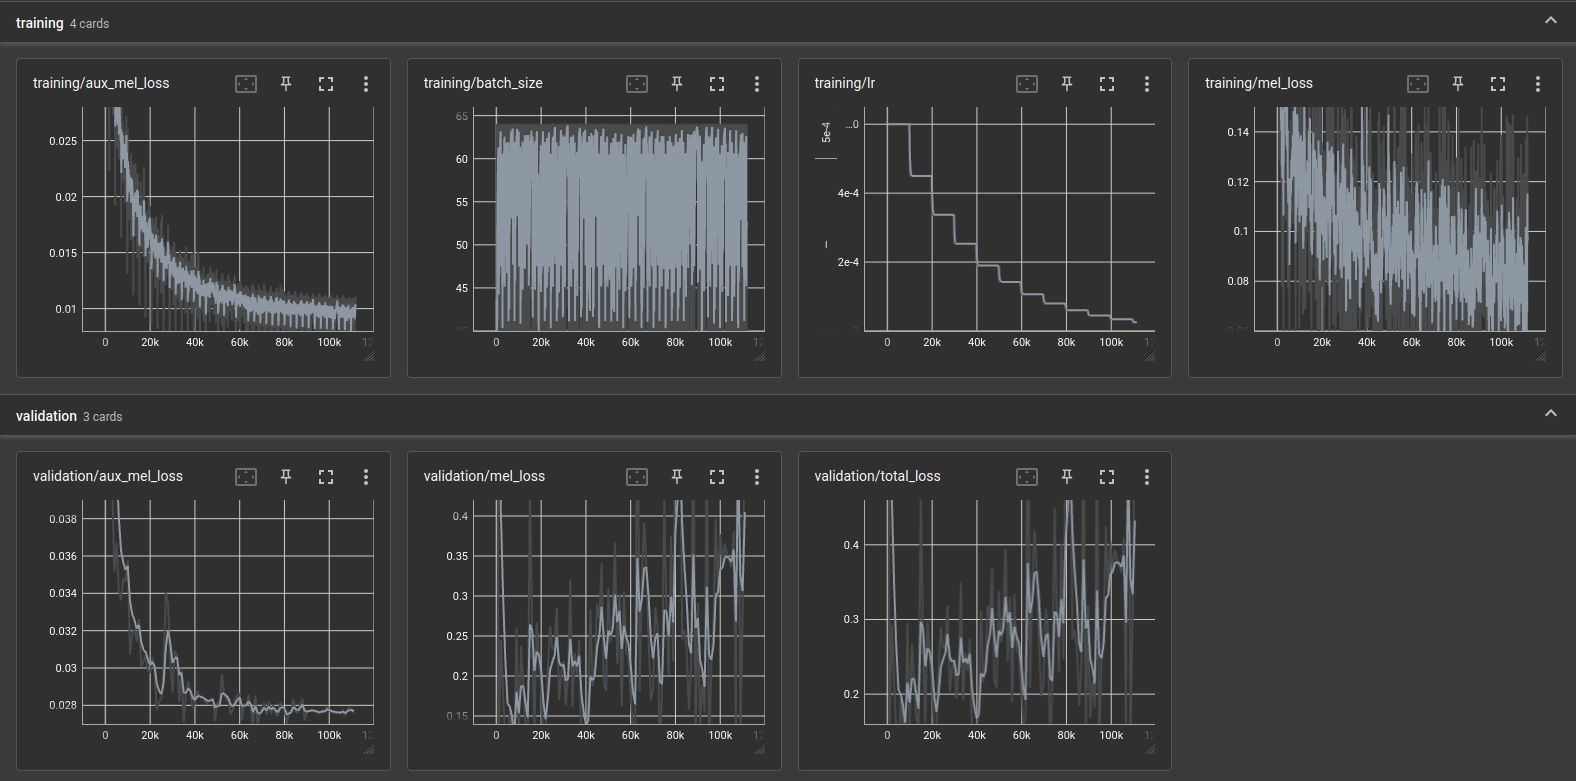
\includegraphics[width=0.5\textwidth]{graphics/v3_training+testing.png}
		\caption{training and validation loss of model 3}
		\label{fig:model3}
	\end{figure}
	
	The idea for the third model was to enlarge the training data size to observe the effect on the model’s performance. So, we extended the data to all available Linkin Parks albums, studio albums as well as live albums but without applying any additional data augmentation techniques. We kept the batch size of 64, but increased the amount of validation samples (now 10) to balance the training validation ratio. The enlarged dataset decelerated the training process massively, reaching 16 hours and 78k epochs of training until the training loss converged. Final loss values comparable to those of the small model were reached during training, minimal value of 0.01 for the training aux mel loss and 0.028 for the validation aux mel loss (see image \ref{fig:model3} ). This model is referred to as large during evaluation. 

	
	\subsubsection{Model 4 (clean)}
	
	\begin{figure}[htbp]
		\centering
		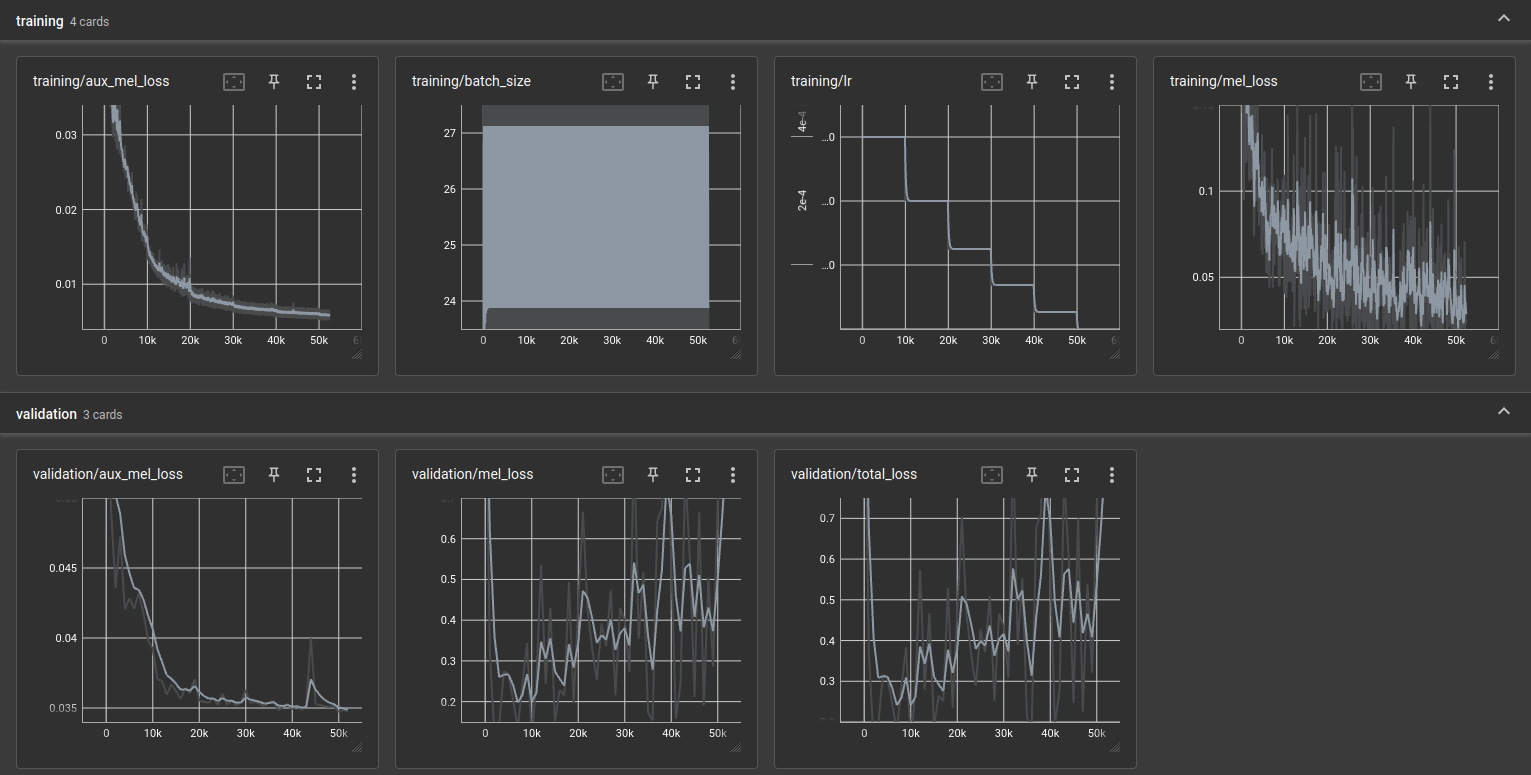
\includegraphics[width=0.5\textwidth]{graphics/v4_training+testing.png}
		\caption{training and validation loss of model 4}
		\label{fig:model4}
	\end{figure}
	
	Next, we generated a clean model, to investigate the relevance of noisy input data on the model performance and audio quality of the results. Therefore we trained the model solely with the reduced hand segmented dataset, that does not contain noisy data or segments with Mike Shinoda’s voice. Due to the smaller dataset we reduced the amount of segments per batch to 64, trained with a lower learning rate of 0.004 and used only 8 samples for validation. Subsequently the duration until loss conversion shrunk to 52k epochs and 6 hours training time. As displayed in image \ref{fig:model4}, the training mel loss reached a minimum of 0.006 and the validation mel loss of 0.03. This model will be referred to as clean.
	
	
	\subsubsection{Model 5 (large+ft+vocoder)}
	
	\begin{figure}[htbp]
		\centering
		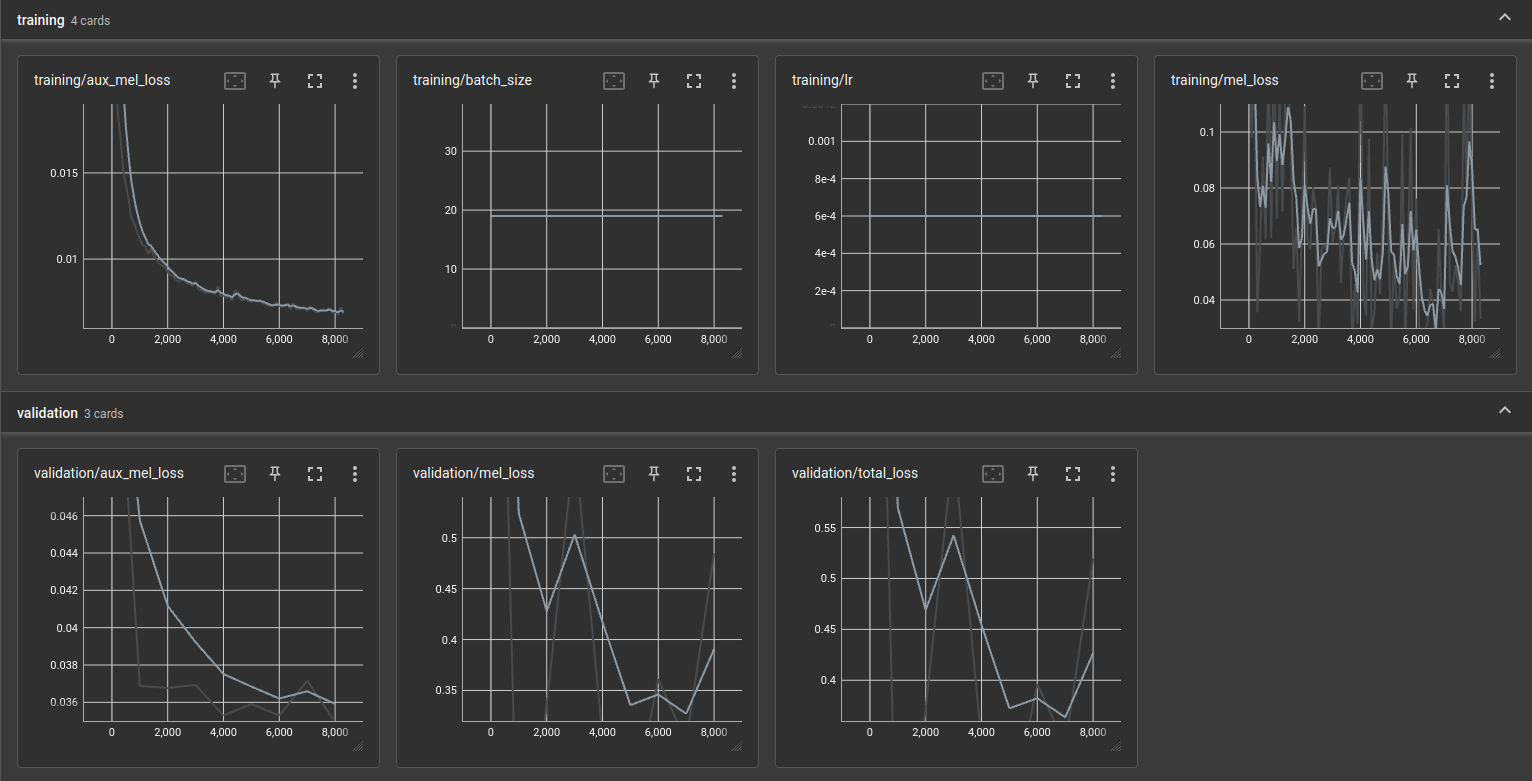
\includegraphics[width=0.5\textwidth]{graphics/v5_training+testing.png}
		\caption{training and validation loss of model 5}
		\label{fig:model5}
	\end{figure}
	
	After probing the relevance of dataset size and data quality, we investigated whether fine-tuning with clean data shows a positive effect. To receive encompassing trends, the fine tuning is also extended to the vocoder. We pretrained the model with the exact same configurations as the large model, though integrated the fine-tuned HifiGAN vocoder instead of the standard vocoder. Following up on the pretraining, where much but low-quality data was used, the model is fine-tuned on the clean dataset to focus on learning the subtle nuances in Chester’s voice. The validation set for the fine-tuning consists of 8 validation samples, all other parameter values were retained from the pretraining. During training, the model confirmed 8000 epochs and ran about 1.5 hours before the validation loss reached convergence. The aux mel training loss minimized to 0.007 and the aux mel validation loss to 0.035 (see image \ref{fig:model5} ). This model will be referred to as ft+vocoder.

	
	\subsubsection{Model 6 (huge+variance+vocoder)}
	
	\begin{figure}[htbp]
		\centering
		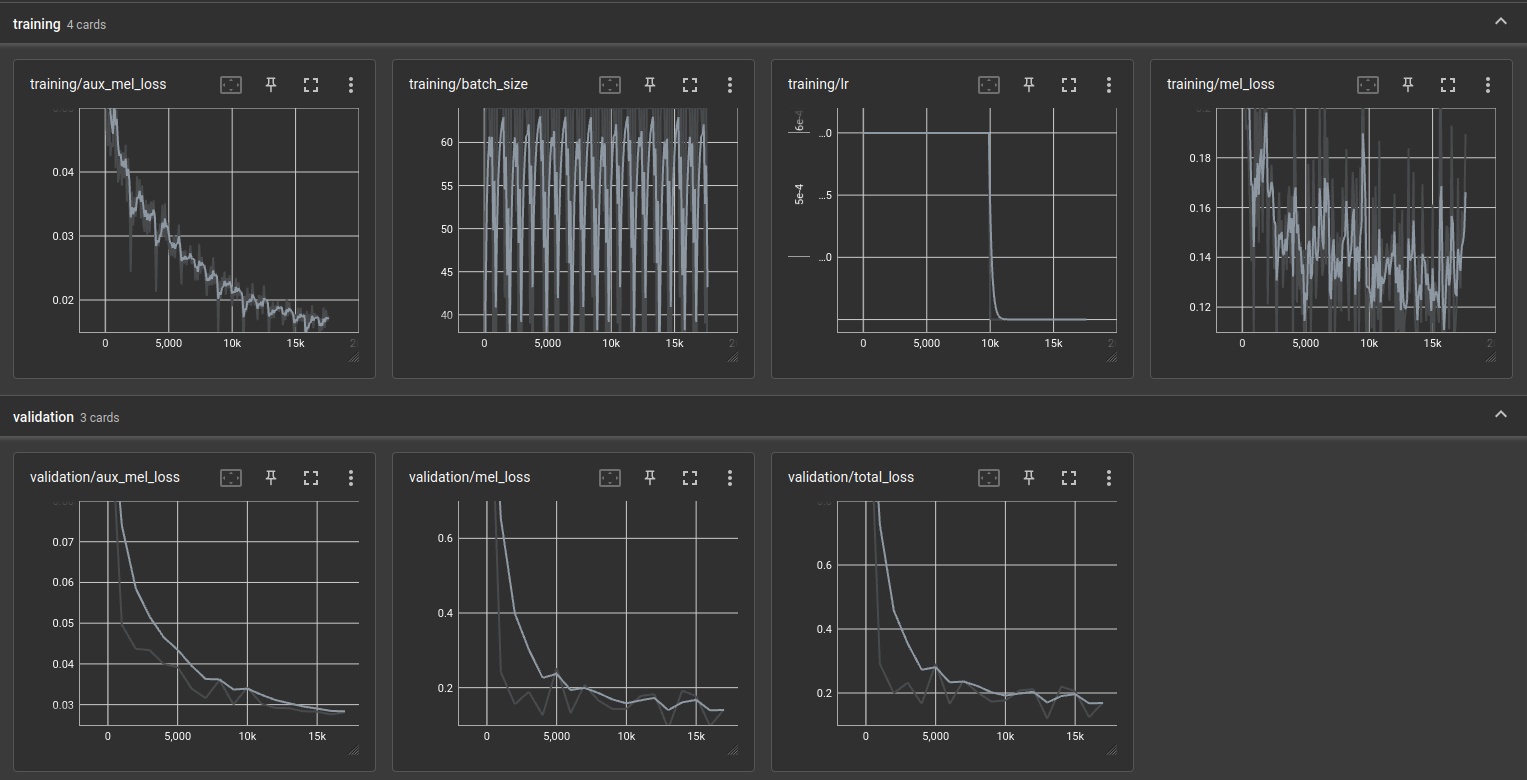
\includegraphics[width=0.5\textwidth]{graphics/v6_training+testing.png}
		\caption{training and validation loss of model 6}
		\label{fig:model6}
	\end{figure}
	
	The task of the variance+vocoder model was to investigate whether the combination of variance and acoustic model is superior over the standard acoustic model and which importance the pitch and tension prediction takes for our experiment. The process is parted into two steps; first we trained the variance model on the large dataset for 11 hours and 97k epochs, then we inferred the large dataset with the variance model and trained the acoustic model on them for 2.5 hours and 17k epochs. The variance model was configured to predict pitch and tension of Chester’s voice. Additionally to the large dataset we further enriched the variance data with the DiffSinger built-in data augmentation method for the acoustic model training.  For both models we integrated the fine-tuned vocoder, used batch size 64  and 10 sample segments for validation. When stopped training the acoustic model achieved a mel aux loss of 0.017 for training and 0.028 for validation (see image \ref{fig:model6} ), further the variance model reached a pitch accuracy of 0.5.
	
	
	\subsubsection{Model 7 (manual + sorted clean)}
	
	\begin{figure}[htbp]
		\centering
		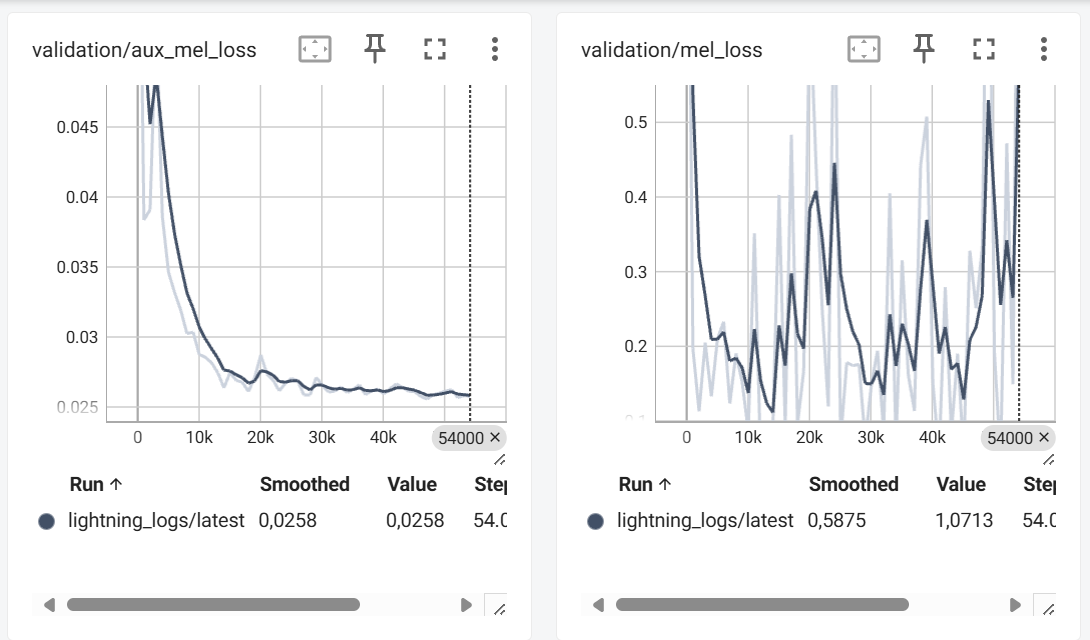
\includegraphics[width=0.5\textwidth]{graphics/v7_testing.png}
		\caption{model 7}
		\label{fig:bild4}
	\end{figure}
	
	As the dataset of the clean model seemed to be too small, we aimed to increase it. However, we wanted to include only “good” audio snippets, therefore, we used some scripts to automatically select other snippets that were considered to be “clean” (see refined preprocessing). This increased the dataset size to more than double the instances compared to the clean model. For this model, we used a batch size of 64 and 8 validation samples. The learning rate was set to 0.006. The model was trained for 54k epochs until the validation loss reached 0.026.
	
	\subsubsection{Model 8 (manual + sorted + augmented clean)}
	
	\begin{figure}[htbp]
		\centering
		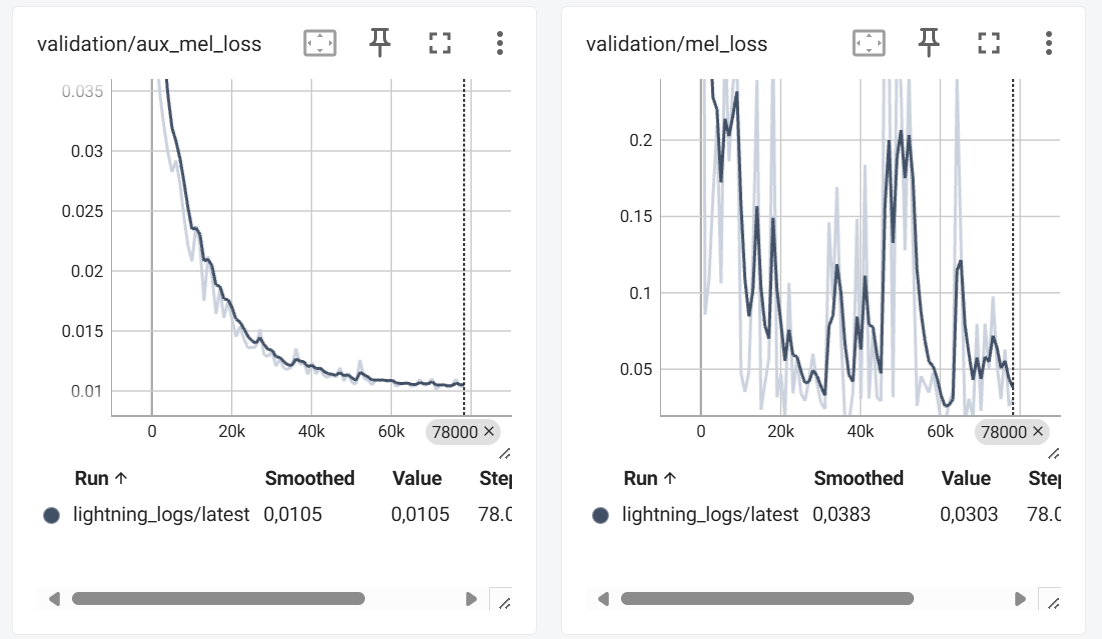
\includegraphics[width=0.5\textwidth]{graphics/v8_testing.png}
		\caption{model 8}
		\label{fig:bild5}
	\end{figure}
	
	As we still wanted to further augment our dataset, we trained the next model with an augmented dataset. We used the segments that we manually selected and those that were selected by the scripts and used different data augmentation techniques, such as pitch shifting, time shifting, noise reduction and loudness shifting (see data augmentation) to artificially enlarge our dataset. The batchsize was set to 64, eight validation samples were used and the learning rate was kept at 0.006. The model was trained for 78k epochs until the validation loss reached almost 0.01.
	
	
	\subsubsection{Model 9 (large + augmented)}
	
	\begin{figure}[htbp]
		\centering
		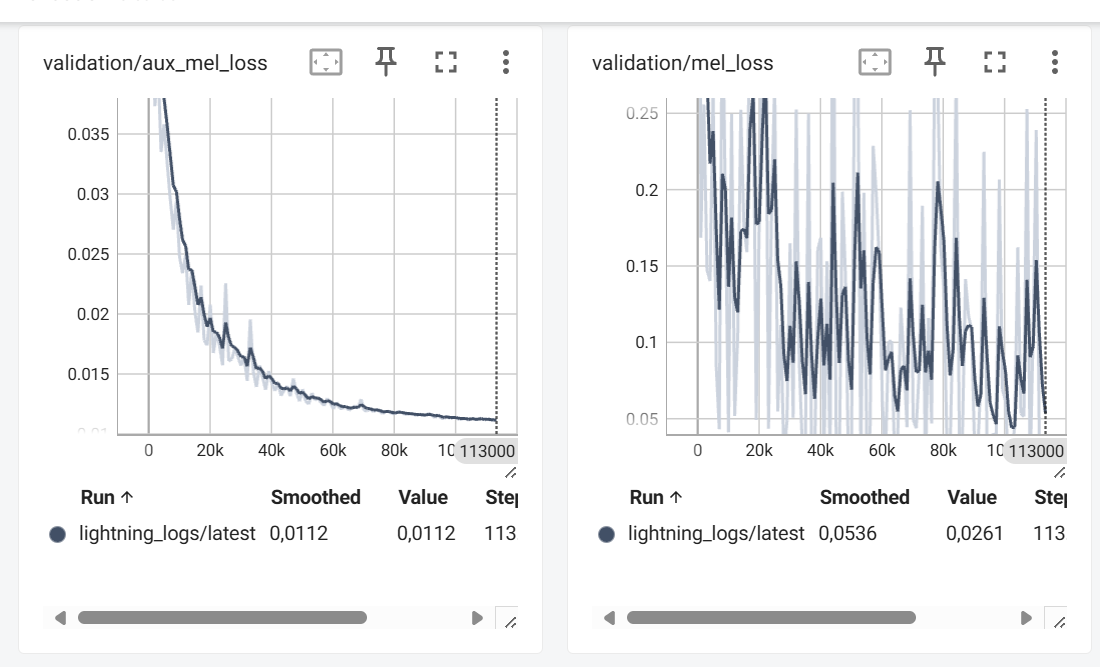
\includegraphics[width=0.5\textwidth]{graphics/v9_testing.png}
		\caption{model 9}
		\label{fig:bild6}
	\end{figure}
	
	Our last attempt was to train a model with data augmentation that included even more data (almost the entire dataset, except for some filtered noise/screams and rap), even though this data included some more overlapping singing and try data augmentation on this model as well. The parameters were kept constant compared to the smaller augmented model. However, this time we used our fine-tuned vocoder. We stopped the training after 113k epochs when it reached a validation loss of 0.011.
	
	\newpage
	
	%==============================================
	%================ Evaluation ===================
	%==============================================
	\section{Evaluation}
	
	\subsection{Choosing a model}
	
	To be able to choose the best model for generating the vocals, we had to
	evaluate them. We chose five different evaluation criteria. These criteria were
	\emph{subjective Mean Opinion Score (MOS-LQS)}, \emph{comparison of histograms
		created from mel spectrograms}, \emph{objective Mean Opinion Score (MOS-LQO) as
		Perceptual Evaluation of Speech Quality (PESQ) score}, the \emph{root mean
		square error of F0 values (F0 RMSE)}, and the \emph{Speech-to-Noise ratio
		(SNR)}. \\
	Each model was evaluated based on these criteria, and compared to the original
	sound files. "gt" in the model lists refer to the \emph{ground truth}, or
	original sound files. The other names refer to the respective model iteration.
	
	\subsection{Used files}
	The following 14 segments were used in the evaluation:
	\begin{itemize}
		\item Segment 22 from album 1, song 4
		\item Segment 3 from album 1, song 5
		\item Segment 1 from album 1, song 8
		\item Segment 22 from album 1, song 8
		\item Segment 5 from album 2, song 4
		\item Segment 7 from album 2, song 6
		\item Segment 17 from album 2, song 6
		\item Segment 1 from album 2, song 9
		\item Segment 7 from album 2, song 9
		\item Segment 3 from album 3, song 5
		\item Segment 13 from album 3, song 5
		\item Segment 1 from album 3, song 6
		\item Segment 10 from album 3. song 6
		\item Segment 8 from album 5, song 3
	\end{itemize}
	
	\subsection{Criteria}
	
	\subsubsection{MOS prediction}
	
	A basic but quite expressive evaluation metric is the mean opinion score (MOS), which originates in the research of telecommunication to assess the quality of human speech. The metric is standardized and quantitative, ranging from values between 0 (worst quality) and 5 (best quality) - where 0 means, communication is not possible despite high efforts and 5 means, communication is afforded effortlessly. 
	
	Previous work, adapted the MOS for voice conversion models, generating automatic mean opinion score prediction models that are now broadly used for voice conversion evaluation. Further applications for automated MOS are for example the detection of artificially generated fake audios or the evaluation of other assessment tools as gold standard. \cite{Zhou2024} However, in the past automated MOS prediction primarily served as a tool to compare different models and model architectures and not for hyperparameter or database testing. Nevertheless, we regard it as a solid basis for further evaluation metrics.
	
	For our project, we integrated the SingMOS model \cite{Tang2024}, a predictor particularly developed for the evaluation of singing voice synthesis models. The collected test dataset consist of 15 segments, purposed to provide a broad coverage of Chester’s different singing styles including screams and shoutings (all segments are as noiseless as possible). The finetune+vocoder and variance+vocoder model were unable to generate inferences of one test segmented, so we left the affected segment out for both models. Additionally we predicted the MOS for the vocal separated audio files to receive a gold standard value - scoring a value of 2.995.
	
	\begin{table}[ht]
		\centering
		\resizebox{\linewidth}{!}{%
		\begin{tabular}{cccccccccc}
			\toprule
			\textbf{Model} & \textbf{gt} & \textbf{small} & \textbf{large} & \textbf{clean} & \textbf{ft + voc} & \textbf{var+voc} & \textbf{man+clean} & \textbf{man+aug} & \textbf{large+aug} \\
			\midrule
			\textbf{MOS} & \textbf{3.00} & 2.74 & 2.83 & 2.76 & 2.77 & \textbf{2.96} & 2.91 & 2.81 & 2.79 \\
			\bottomrule
		\end{tabular}
		}
		\caption{average MOS predictions across different models}
		\label{tab:mos_scores}
	\end{table}
	
	All results are averaged across the models and summarized in table \ref{tab:mos_scores}. As expected none of the models surpasses the ground truth value of the vocal separated segments. Additionally the distance between the highest and lowest performing model is with 0.22 score points difference only marginal. 
	
	The variance+vocoder model outperformed all other models and reached results comparable to the ground truth, indicating outputs with relatively high audio quality. At some distance follows the result of the manual+clean model, achieving a slightly worse but still comparably high predicted MOS score. What is striking is that in particular models trained on smaller datasets (independent of audio quality) seem to receive lower MOS prediction values. We suspect this trend to be provoked by noise in the output audios.
	
	\subsubsection{Histogram Comparison}
	
	In the next step, we wanted to evaluate the models based on a comparison of the mel spectrograms. A recent blog post introduced a method, where the mel spectrograms are converted to histograms (distribution of the bin values), which are easier to compare. \cite{mel-spectrogram} This approach resembles the comparison of the underlying bin distribution and therefore takes the place of a meta evaluation. 
	
	To measure the difference of the generated histograms, we applied several common comparison metrics. First measurement is the Correlation of both histograms, with values ranging from -1 (totally uncorrelated) to 1 (totally correlated) - which draws an extremely direct connection between both bin distributions. Another popular measurement to compare histograms and distributions in general is the Chi-Square distance. Strength of the metric is the sensitivity for large distances, meaning distributions that deviate strongly from the original histogram can be detected easily and filtered out. Obtained values range from 0 to infinity, the larger the value the more mismatches the distribution. A completely different perspective allows the Intersection measure of the histograms, where the overlapping of equal bin values is computed. With the comparatively low complexity and computational cost comes quite inaccurate results, that might be fluctuating and less expressive for model performance. The higher the Intersection value, the more bin values share two distributions. A more refined measurement is the Bhattacharyya distance, which originates in the measurement of probability distribution similarity. Similar to the Chi-Square distance, the smaller the value, the higher is the distribution’s similarity. 
	
	\begin{table}[ht]
		\centering
		\resizebox{\linewidth}{!}{%
			\begin{tabular}{cccccccccc}
				\toprule
				Model & gt & small & large & clean & ft+voc & var+voc & man+clean & man+aug & large+aug \\
				\midrule
				MOS ↑           & \textbf{3.00} & 2.74 & 2.83 & 2.76 & 2.77 & \textbf{2.96} & 2.91 & 2.81 & 2.79 \\
				Correlation ↑   & --   & \textbf{0.94} & 0.94 & 0.92 & 0.93 & \textbf{0.95} & 0.93 & 0.94 & 0.93 \\
				Chi-Square ↓    & --   & \textbf{248394} & \textbf{298899} & 805762 & 649244 & 575705 & 839064 & 578248 & 360068 \\
				Intersection ↑  & --   & 120777 & \textbf{122109} & 118189 & 119622 & \textbf{122664} & 119577 & 121230 & 121170 \\
				Bhattacharyya ↓ & --   & 0.20 & 0.21 & 0.21 & 0.18 & \textbf{0.16} & 0.18 & 0.18 & \textbf{0.17} \\
				\bottomrule
			\end{tabular}
		}
		\caption{averaged scores of the historgram similarity to ground-truth across different models}
		\label{tab:quantitative_eval}
	\end{table}
	
	We implemented all metrics quoted above and tested them on the entirety of our models, using the same test set as for the MOS prediction. Each model is compared with the vocal separated data as our gold standard. The obtained results are averaged for each model and summarized in table \ref{tab:quantitative_eval}. 
	
	The variance+vocoder model outperforms all other models, achieving constant and strong results in almost every comparison measurement, indicating a clear dominance between the tested models. 
	For the Correlation values we observe just minor differences, but the variance+vocoder model and the large model achieve the highest results with scores around 0.95. 
	
	While keeping in mind that the Intersection value might possibly be less informative than other comparison measurements, the variance+vocoder and large model again achieve the highest results, with the most overlapping of bin values. Furthermore, models trained or fine-tuned on the clean dataset perform the worst with this metric. Potentially, the “high quality” data is shifting or skewing the results in either direction, which preserves general distribution properties but changes the bin overlap.
	
	The Chi-Square distance remains the only measurement, where the variance+vocoder model is beaten by other models - with the small and large model outperforming the rest, both reaching values below 300000. However, no enlightening tendencies or correlations between model hyperparameters and Chi-square distance are observable, therefore the values appear to be rather meaningless for the evaluation.
	The variance+vocoder model scores the smallest Bhattacharyya distance with the value 0.16, once more outperforming all other tested models. In general models with the fine-tuned vocoder reached comparatively good results, where further research is necessary to investigate potential reasons for this effect.
	
	\subsubsection{Perceptual Evaluation of Speed Quality (PESQ)}
	While the evaluation using SingMOS is considered a subjective evaluation, PESQ
	is an objective Mean Opinion Score evaluation. The result of PESQ is usually a
	score of the perceived speech quality on a scale of 1.0 to 4.5 (with narrowband,
	4.64 with wideband), with a value of <2.0 representing a poor perceived speech
	quality, which may be hard to understand. A value of about 3.0 is considered a
	fair quality with some degradation, but generally understandable, and a value of
	4.0 or more is considered excellent quality, with (almost) no degradation.
	Although PESQ itself aligns both input files to account for timing mismatches,
	it should be irrelevant in our case, as both input files are supposed to have
	the same text, and everything was already aligned previously. The perceptual
	part in PESQ refers to the way the sound files are analyzed. Instead of treating
	every frequency and loudness the same, PESQ mimics the human ear and how an ear
	is more sensitive to certain frequencies. The reference value for identical
	files (comparing the original sound files with themselves), is approximately 4.64, as
	expected.
	
	\subsubsection{PESQ results}
	\begin{figure}[hbtp]
		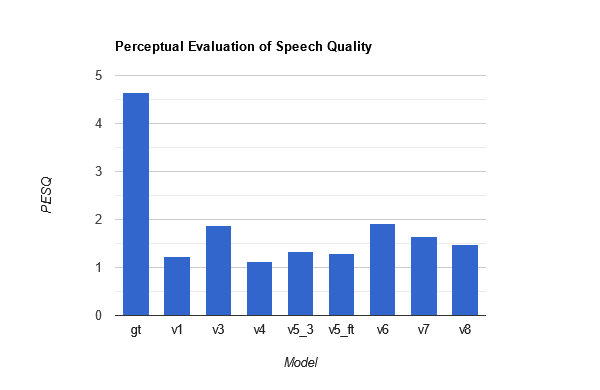
\includegraphics[width=\textwidth]{evaluation/graphs/PESQ.png}
		\caption{Perceptual Evaluation of Speech Quality results per model}
		\label{fig:pesq_results}
	\end{figure}
	
	Figure \ref{fig:pesq_results} shows the results of the PESQ evaluation on each
	model. The first bar with a value of 4.64 is the reference value with a perfect
	score. The graph clearly shows that the models we evaluated do not come close to
	what is considered an excellent result in PESQ. The best models according to
	PESQ are the large and the manual+sorted clean model.
	
	\subsubsection{F0 Root mean square error (F0 RMSE)}
	The F0 value of speech, often also referred to as pitch or fundamental
	frequency, is measured in Hertz, and describes the rate of vibration of the
	vocal folds. The range of F0 is usually between 50 Hz to 450 Hz. This evaluation
	compares the extracted F0 values from the original sound files to the ones
	generated with each model. With the resulting differences, the root mean square
	error is calculated to be able to assign each model a single score value. When
	comparing specific extracted values of sound files, it is usually needed to use
	dynamic time warping (DTW) to match the corresponding values to each other. In
	our case this was not needed, as we already aligned each file using DTW before.
	The reference value when comparing the original sound files with themselves, is
	0.0 as there is no difference between them and therefore no error.
	
	\subsubsection{F0 RMSE results}
	\begin{figure}[hbtp]
		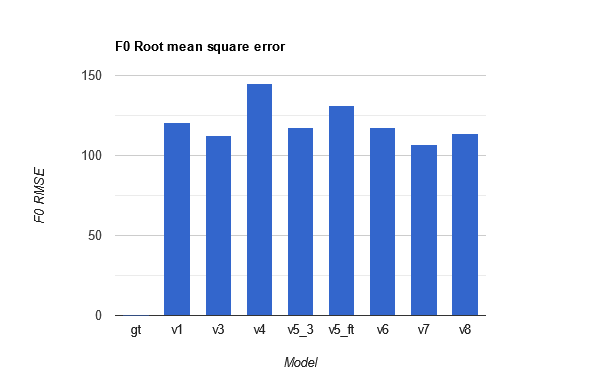
\includegraphics[width=\textwidth]{evaluation/graphs/F0RMSE.png}
		\caption{Fundamental frequency root mean square error}
		\label{fig:f0rmse_results}
	\end{figure}
	
	The chart in figure \ref{fig:f0rmse_results} shows the root mean square error of
	the fundamental frequency, sometimes also referred to as pitch, for each model
	we used. The shown reference value of 0.0 for \emph{gt} is a perfect value and
	therefore usually not achieved in real calculations.
	
	\subsubsection{Speech-to-Noise ratio (SNR)}
	The Speech-to-Noise ratio (SNR) compares the ratio of speech in a sound file, to
	the amount of background noise. The formula used in this evaluation is \\
	\[
	SNR = 10*log_{10} (\frac{RMSE(signal)}{RMSE(noise)})
	\]
	as formulated in \cite{ji2020comprehensivesurveydeepmusic}. The SNR is equal to 10 times the 10th log of the RMSE of
	the original file (signal) divided by the RMSE of the generated file (noise). It
	is usually measured in decibels (dB). The reference value for a perfect ratio is
	0.0 as shown by comparing the original sound files to themselves.
	
	\subsubsection{SNR results}
	\begin{figure}[hbtp]
		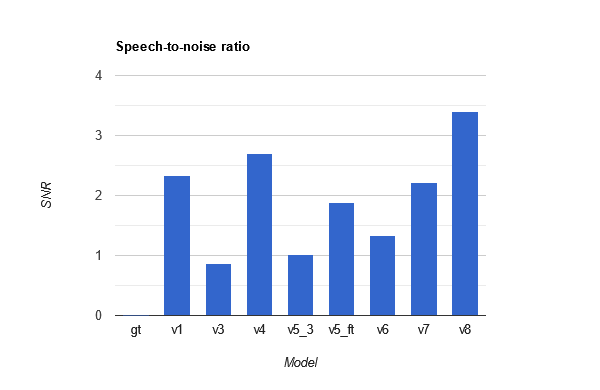
\includegraphics[width=\textwidth]{evaluation/graphs/SNR.png}
		\caption{Speech-to-noise ratio}
		\label{fig:snr}
	\end{figure}
	
	While SNR usually refers to Signal-to-noise ratio, and describes the ratio of
	the wanted signal, and background noise, in our case it refers to
	Speech-to-noise ratio. It describes the ratio of speech to background noise.
	Figure \ref{fig:snr} shows the reference value of 0.0 for the ground truth and
	the respective values for the used models. In this case the large model is the
	best one according to the SNR.
	
	\newpage
	
	%==============================================
	%============= Mixing and Mastering ============
	%==============================================
	\section{Mixing and Mastering}

	The vocal track generated by DiffSinger posed some challenges during mixing. Inconsistent tones, robotic artifacts and a lack of natural dynamics all required extensive processing to attempt to improve its quality. Indeed, the output track contains glitches, sudden pitch shifts, muffled consonants and irregular sustain. The sustained notes sound unnaturally flat and lack vibrato. To address this, we first tried to trim segments and applied noise reduction using ReaFIR. A high-pass filter at 120 Hz (ReaEQ) removed the jarring low-frequency rumble. Given the irregular dB dynamics where some words were overly loud and others nearly inaudible. We automated a +2 dB rise during the chorus to compensate for the model’s weak projection on longer notes. To make up for some synthetic artifacts, we applied a cut at 2–3 kHz (-5 dB, Q=4) to reduce the volume of some harsh resonances. We then added a high-shelf boost at 8 kHz (+2 dB) for added clarity to handle occasional muffled sibilants. Moreover, compression was used to stabilize the uneven output and an even dB level. ReaComp set at 4:1 ratio, 20 ms attack, 100 ms release provided 6 dB of gain reduction to lower some peaks. We also used  a limiter (ReaLimit) to prevent the track from clipping. To account for the “s” and “t” sounds, we used the FabFilter PRO-DS vst-plugin. However, despite these efforts, the vocals retained an unnatural texture, which we attempted to mitigate, by applying some saturation, not just to add warmth, but also to Emulate Emily Armstrong’s raspy tone that the model failed to emulate. 
	Mastering
	In music production, mastering is the final stage before the release of a song or an album. The process consists of mixing and polishing the master track that comprises all single tracks in order to achieve consistency, optimal loudness and compatibility across various playback systems. Unlike mixing, which focuses on balancing individual tracks (vocals, instruments), mastering addresses the entire stereo mix as a single unite. Indeed, this phase aimed to unify the mix’s tonal balance and loudness. Thus, some EQ (FabFilter Pro-Q3) was applied to the stereo bus to mitigate the harshness at 3.5 kHz (-1.5 dB, Q=2) and add a touch of higher frequency with a high-shelf boost at 12 kHz (+1 dB). Multiband compression (FabFilter - MB) was applied to tighten the low-midrange (200–500 Hz) and reduce the “muddiness” that stems from the vocal’s uneven low-end resonance. Finally a limiter (FabFilter-L2) was set to +9 to boost loudness in accordance with modern rock and metal commercial standards.

	
	\newpage
	
	%==============================================
	%================ Conclusion ===================
	%==============================================
	\section{Conclusion}
	
	The goal of our project was to develop an SVS model that could replicate the unique voice of Chester Bennington. Our approach focused not just on the training itself, but on creating a comprehensive pipeline that would allow others to have a guide that covers everything from data processing, data augmentation, training, evaluation and post-processing of the data to be able to use DiffSinger with their own data. So our intention is not just to create a replica of Chester's voice, but to provide an understandable guide to creating a DiffSinger model.
	
	After creating our dataset with the unprocessed audio, we began pre-processing, an important step that determines the quality of our model. The first step was to extract the vocals to ensure that the model was only trained on relevant vocal data. This was followed by the segmentation and alignment of the data, as well as the creation of ds-files, which are needed for the use of DiffSinger.
	
	This first preprocessing was followed by a second, which focussed on improving the quality of the data. For this purpose, some songs were edited manually so that disturbing noises and inappropriate sequences (e.g. wrong singer) were cut out. Some scripts also filtered out faulty segments. The alignment and ds-file creation steps were then repeated.
	
	For the data augmentation process, we explored both DiffSinger's built-in augmentation functions and manual augmentation methods. While the built-in methods included pitch shifting and time stretching, we also applied pitch shifting, volume adjustment, noise reduction and velocity change to simulate real-world variations in vocal performance.
	
	
	Setting up the training presented us with some challenges in terms of configuring the environment, setting up the hardware and dealing with outdated documentation. We initially tried to use Docker, but ran into issues with the module locations, so we decided to switch to a more reliable Anaconda environment. Once we had configured our system, we trained our models on the LST servers at Saarland University using HTCondor to schedule training jobs. The training progress was monitored with TensorBoard.
	
	We trained different models experimenting with different parameters such as the size of the dataset, different quality of the dataset, the use of data augmentation, different vocoders and different learning rate and fine-tuning settings.
	
	
	Despite extensive experimentation, the overall model performances remain relatively close. While some vocal segments are handled well by most models, others result in distorted, rough-sounding outputs or noticeable background noise. Common issues that we encounted during inference include misaligned or incorrect phonemes and inconsistent transitions. To quantify the model performances, we used five evaluation methods: predicted Mean Opinion Score (MOS) via SingMOS, mel-spectrogram histogram comparisons, objective MOS using PESQ, F0 Root Mean Square Error (F0 RMSE), and Speech-to-Noise Ratio (SNR). The variance+vocoder model revealed the best MOS scores and a strong spectral similarity to real vocals. The manual+sorted clean model achieved the best results for PESQ. Model 8 (manual+sorted+augmented clean) achieved the best results in the F0 RMSE evaluation and the large model achieved the best results for the SNR evaluation. This shows that the models have different strengths and weaknesses and in the end achieved quite similar results. Even the top-performing models could not fully replicate the expressive detail and clarity of the original vocals, often struggling with distorted phonemes, rough transitions, or alignment errors. 
	
	A probable issue could be the automatic alignment. To address this problem, aligning the data manually would almost certainly lead to a better model as many boundaries are inadequate. However, this step requires a non-negligible amount of time, offering potential for future research. There can also be made improvements within the data augmentation as the project has highlighted the importance of careful and balanced augmentation to avoid degrading the model’s performance. Aquiring enough high-quality data is a challenging task considering that Chester Bennington is dead and the amount of data, therefore, limited. However, when transferring our approach to modelling the voice of another singer, collecting more high-quality data is crucial for obtaining convincing results.
	
	Our last step was the mixing and mastering. As the DiffSinger-generated vocals exhibited robotic artifacts, pitch shifts, and a lack of natural dynamics, we used noise reduction, EQ adjustments, dynamic automation, compression, limiting, de-essing, and saturation to improve clarity and emulate a raspy vocal tone. During the mastering, EQ and multiband compression balanced harshness and muddiness, while a limiter boosted loudness to match commercial rock and metal standards. 
	
	The main contribution of this project is the creation of a comprehensive guide for setting up and training a DiffSinger model, from data pre-processing to fine-tuning the model and post-processing. By documenting each stage of the process, we provide a valuable resource for others who wish to emulate or improve upon our work in speech synthesis. This guide serves as a step-by-step reference for anyone interested in training a speech synthesis model with DiffSinger, covering not only technical details, but also the challenges we encountered and how they were overcome.
	
	
	To summarise, this project has provided valuable insights into the use of DiffSinger for voice replication, particularly in terms of data pre-processing, augmentation, model setup and post-processing. Our project also highlights the shortcomings of the results, which are mainly due to poor alignment and insufficiently high-quality data (e.g. an insufficient number of acapellas).  Therefore, further refinements are needed to fully capture the nuances of a unique voice like Chester Bennington's. Nonetheless, our efforts have established a solid foundation for future research and development in the field of voice synthesis, with the guidelines presented here providing a robust framework upon which others can build.
	
	%==============================================
	%================ Sources ===================
	%==============================================
	
	\newpage
	\bibliographystyle{plain}  % This style sorts references alphabetically
	\bibliography{references}  % This will load your references.bib file
	
	
	
\end{document}

